% !TEX program = pdflatex
% !TeX encoding = utf8
% !TeX spellcheck = pl-PL

%%%%%%%%%%%%%%%%%%%%%%%%%%%%%%%%%%%%%%%%%%%%%%%%%%%%%%%%%%%%%%%%%%%%%%%%%%%
% Wybierz rodzaj pracy dyplomowej oraz wydział
% Pick thesis type and faculty
%%%%%%%%%%%%%%%%%%%%%%%%%%%%%%%%%%%%%%%%%%%%%%%%%%%%%%%%%%%%%%%%%%%%%%%%%%%
\documentclass[thesis=inz,faculty=ee]{EE-dyplom} 

% thesis=[inz|mgr|bsc|msc]
%  * inz - praca inżynierska
%  * mgr - praca magisterska
%  * bsc - bachelor thesis
%  * msc - master thesis

% Skróty nazw wydziałów zgodne z domenami internetowymi
% faculty=[arch, gik, ee, wip]

%%%%%%%%%%%%%%%%%%%%%%%%%%%%%%%%%%%%%%%%%%%%%%%%%%%%%%%%%%%%%%%%%%%%%%%%%%%
% Konfiguracja - do personalizacji
% Configuration - to be personalized
%%%%%%%%%%%%%%%%%%%%%%%%%%%%%%%%%%%%%%%%%%%%%%%%%%%%%%%%%%%%%%%%%%%%%%%%%%%
\instytut{Instytut Elektrotechniki Teoretycznej i Systemów Informacyjno-Pomiarowych}
\kierunek{Automatyka i Robotyka Stosowana}
\specjalnosc{Systemy Wbudowane}
\title{Projekt i implementacja systemu wbudowanego z asymetrycznym przetwarzaniem wielordzeniowym}
\engtitle{Design and implementation of an embedded system with asymmetric multiprocessing}
\album{331797}
\author{Beniamin Raczyński}
\promotor{dr inż. Makowski}
\date{2026}
\longdate{2026-04-02}

%%%%%%%%%%%%%%%%%%%%%%%%%%%%%%%%%%%%%%%%%%%%%%%%%%%%%%%%%%%%%%%%%%%%%%%%%%%
% Streszczenie pracy i abstract.
% In case of thesis in English swap the order - English version goes first.
%%%%%%%%%%%%%%%%%%%%%%%%%%%%%%%%%%%%%%%%%%%%%%%%%%%%%%%%%%%%%%%%%%%%%%%%%%%
\streszczeniepracy{
Niniejsze sprawozdanie opisuje proces projektowania i implementacji systemu wbudowanego opartego na architekturze AMP (ang. Asymmetric Multiprocessing). W ramach projektu skonfigurowano środowisko pracy z dostępem VPN (Tailscale), skompilowano system operacyjny Linux oraz wydzielono zasoby procesora dla kodu działającego w trybie bare-metal. Omówiono mechanizmy komunikacji IPC oraz integrację sprzętu poprzez drzewo urządzeń (Device Tree).
} % koniec streszczenia

\slowakluczowe{SoC, Linux, Bare-metal, AMP, IPC, Device Tree, Tailscale}

\thesisabstract{
This project report describes the design and implementation of an embedded system based on AMP (Asymmetric Multiprocessing) architecture. The project involved configuring a development environment with VPN access (Tailscale), compiling the Linux operating system, and isolating processor resources for code running in bare-metal mode. IPC communication mechanisms and hardware integration via the Device Tree are discussed.
} % end of abstract

\thesiskeywords{SoC, Linux, Bare-metal, AMP, IPC, Device Tree, Tailscale}

%%%%%%%%%%%%%%%%%%%%%%%%%%%%%%%%%%%%%%%%%%%%%%%%%%%%%%%%%%%%%%%%%%%%%%%%%%%
% Tu zaczyna się dokument
% Here is the beginning of the document
%%%%%%%%%%%%%%%%%%%%%%%%%%%%%%%%%%%%%%%%%%%%%%%%%%%%%%%%%%%%%%%%%%%%%%%%%%%
\begin{document}
    % Strony nagłówkowe - musi być
    % Headers - must exist
    \frontpages
    
    % Tekst pracy - osobne pliki do edycji
    % Thesis text - separate files for edition

    \chapter{Wstęp}
\label{ch:wstep}

Rozwój nowoczesnych układów SoC (ang. \textit{System on a~Chip}) pozwala na łączenie bogatych systemów operacyjnych, takich jak Linux, z~systemami czasu rzeczywistego w~ramach jednej jednostki krzemowej. 

Celem niniejszej pracy jest zaprojektowanie i~wdrożenie architektury asymetrycznego przetwarzania wielordzeniowego (AMP). Praca obejmuje przygotowanie pełnego stosu technologicznego: od środowiska programistycznego, przez opis sprzętu (Device Tree), po własne sterowniki i~aplikacje bez systemu operacyjnego (ang. \textit{bare-metal}).

W kolejnych rozdziałach przedstawiono szczegółowo proces zestawienia platformy badawczej oraz kroki realizacyjne projektu.

    \chapter{Przygotowanie stanowiska pracy i~infrastruktury}
\label{ch:stanowisko}

Realizacja złożonych projektów dla systemów wbudowanych wymaga przygotowania elastycznego i~bezpiecznego środowiska pracy. W~tym rozdziale opisano konfigurację sieciową oraz interfejsy dostępowe do sprzętu.

\section{Dostęp zdalny z~wykorzystaniem sieci VPN Tailscale}
Aby umożliwić bezproblemowy dostęp do serwera kompilacyjnego oraz fizycznej platformy sprzętowej bez konieczności posiadania publicznego adresu IP, wykorzystano sieć opartą na technologii WireGuard -- Tailscale. Rozwiązanie to pozwoliło na utworzenie bezpiecznej sieci wirtualnej (ang. \textit{mesh VPN}).

\section{Komunikacja szeregowa i~interfejs USB Blaster}
Do niskopoziomowej komunikacji z~układem SoC wykorzystano komunikację szeregową (UART). Programowanie części sprzętowej (FPGA) oraz bezpośredni dostęp do procesora zrealizowano za pomocą interfejsu USB Blaster.

    \chapter{Architektura systemu operacyjnego i~podział zasobów}
\label{ch:architektura}

Głównym założeniem architektonicznym projektu było rozdzielenie zadań pomiędzy dostępnymi rdzeniami procesora. 

\section{Wydzielenie rdzenia z~systemu Linux (Core Isolation)}
Aby zapewnić przewidywalny czas wykonywania dla kodu bare-metal, system Linux musiał zostać pozbawiony kontroli nad jednym z~rdzeni CPU. Zrealizowano to za pomocą argumentów linii komend jądra (np. parametr \texttt{isolcpus}), co uchroniło dany rdzeń przed standardowym planistą (ang. \textit{scheduler}) systemu operacyjnego.

\section{Mechanizmy komunikacji międzyprocesorowej (IPC)}
Komunikacja pomiędzy systemem Linux uruchomionym na głównym klastrze rdzeni, a~kodem bare-metal działającym na rdzeniu wydzielonym, wymagała niezawodnego mechanizmu IPC (ang. \textit{Inter-Processor Communication}). Wykorzystano do tego bloki pamięci współdzielonej (Shared Memory) oraz przerwania sprzętowe typu IPI (ang. \textit{Inter-Processor Interrupt}).

    \chapter{Kompilacja systemu wbudowanego}
\label{ch:kompilacja}

Rozdział ten opisuje proces dostosowania oraz budowy dedykowanego obrazu jądra systemu operacyjnego Linux i~docelowego systemu plików (ang. \textit{rootfs}). Z~uwagi na konieczność maksymalnej optymalizacji, pozbycia się zbędnego oprogramowania (tzw. \textit{bloatware}) oraz specyfikę rozwiązań czasu rzeczywistego, w~projekcie zrezygnowano z~wykorzystania standardowych, desktopowych dystrybucji (takich jak Ubuntu). Zamiast tego zdecydowano się na wygenerowanie środowiska operacyjnego ściśle dopasowanego do założeń sprzętowych.

\section{System plików Yocto Project}
Aby stworzyć maksymalnie zoptymalizowane, lekkie i~wolne od narzutu zbędnych usług środowisko uruchomieniowe, zastosowano system budowania Yocto Project. Obecnie wykorzystano fundamentalną dystrybucję referencyjną Poky, co pozwoliło na znaczne zmniejszenie rozmiaru partycji \textit{rootfs} i~zagwarantowało wysoką wydajność systemu w~kontekście aplikacji czasu rzeczywistego (RT, ang. \textit{Real-Time}). Rozwiązanie to stanowi stabilną bazę i~pozostawia ogromne pole do dalszego, modułowego rozwoju (np. poprzez dodawanie nowych warstw i~pakietów) w~kolejnych etapach życia projektu.

\section{Struktura repozytorium i~źródła jądra systemu}
Płytka ewaluacyjna Terasic DE25 Nano oparta o~układ Intel Agilex 5 stanowi wysoce specyficzną platformę sprzętową (ang. \textit{custom hardware}), dla której standardowe jądro (ang. \textit{vanilla kernel}) nie zawiera wystarczającego wsparcia. Aby zagwarantować pełną kompatybilność sprzętową, konieczne było wykorzystanie jądra dostarczanego bezpośrednio przez producenta.

W~tym celu wykonano rozgałęzienie (ang. \textit{fork}) oficjalnego repozytorium \texttt{linux-socfpga} firmy Terasic. Repozytorium to zostało zintegrowane z~głównym katalogiem roboczym całego projektu przy wykorzystaniu mechanizmu submodułów (ang. \textit{Git submodules}). Zastosowanie takiego rozwiązania pozwala na wygodne śledzenie zmian w~kodzie producenta, a~jednocześnie umożliwia pełną kontrolę nad własnymi modyfikacjami, na które złożyła się m.in. implementacja łaty czasu rzeczywistego \texttt{PREEMPT\_RT} oraz włączenie wsparcia dla wymaganych komponentów sprzętowych.

\section{Konfiguracja jądra Linux i~środowisko kompilacji}
Proces konfiguracji jądra (Kconfig) został przeprowadzony w~celu włączenia obsługi dedykowanych mechanizmów sprzętowych. Korzystając z~interfejsu \texttt{menuconfig}, do głównego drzewa dodano między innymi obsługę sterownika układu AMC6821, który pełni na płytce funkcję sprzętowego monitora parametrów oraz inteligentnego kontrolera wentylatora. Wynikowa konfiguracja została zapisana do pliku \texttt{defconfig}, gwarantując powtarzalność procesu kompilacji.

Proces budowania obrazu \texttt{Image} jest realizowany przy pomocy narzędzi do kompilacji skrośnej (ang. \textit{cross-compilation toolchain}) dla architektury ARM64 (\texttt{aarch64-linux-gnu-gcc}). Aby zapewnić spójność środowiska budowania, główne zmienne systemowe definiujące ścieżki i~narzędzia ujęto bezpośrednio w~głównym pliku \texttt{Makefile} projektu:

\begin{lstlisting}[language=make, caption={Fragment pliku Makefile definujący zmienne dla kompilacji skrośnej}, label={lst:makefile_cross}]
export ARCH ?= arm64
export CROSS_COMPILE ?= aarch64-linux-gnu-

export KDIR := $(CURDIR)/linux-source
export INCLUDE_DTS := $(KDIR)/arch/arm64/boot/dts/intel
\end{lstlisting}

Wyeksportowanie zmiennej \texttt{KDIR} wskazującej na zmodyfikowane i~skompilowane źródła jądra jest kluczowe dla dalszych etapów projektu. Pozwala to na bezpośrednie i~bezkonfliktowe budowanie własnych, zewnętrznych modułów jądra (sterowników \texttt{.ko}) oraz kompilację drzewa urządzeń (ang. \textit{Device Tree}, pliki \texttt{.dtb}), gwarantując, że zostaną one skonsolidowane z~dokładnie tym samym wydaniem jądra, które zostanie uruchomione na platformie docelowej.

\begin{figure}[htbp]
    \centering
    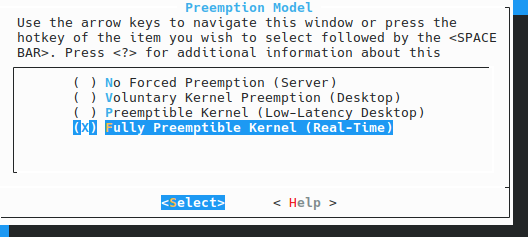
\includegraphics[width=0.75\textwidth]{rysunki/kconfig.png} % Dostosuj ścieżkę do swojego pliku
    \caption{Widok interfejsu narzędzia \texttt{menuconfig} przedstawiający aktywację w~pełni wywłaszczalnego jądra czasu rzeczywistego (łata PREEMPT\_RT).}
    \label{fig:kconfig_rt}
\end{figure}
    \chapter{Opis sprzętowy i~drzewo urządzeń (Device Tree)}
\label{ch:sprzet_dtb}

W nowoczesnych systemach osadzonych opartych na architekturze ARM, informacja o~fizycznie podłączonych peryferiach jest przekazywana do jądra operacyjnego w~postaci struktury zwanej drzewem urządzeń (ang. \textit{Device Tree})[cite: 12]. Stanowi ono sprzętową mapę, która uniezależnia kod skompilowanego jądra od konkretnej topologii płyty bazowej.

\section{Struktura pliku DTS i~rezerwacja pamięci}
Na potrzeby projektu utworzono i~zmodyfikowano pliki źródłowe \texttt{.dts} i~\texttt{.dtsi}[cite: 13]. W~pliku nadrzędnym \texttt{socfpga\_agilex5\_de25\_nano.dts} zadeklarowano włączenie (\textit{include}) plików bazowych dla SoC Agilex 5. 

Kluczowym elementem implementacji było utworzenie węzła \texttt{/reserved-memory}. Opisano w~nich m.in. zarezerwowane obszary pamięci dla rdzenia bare-metal[cite: 13]. Przestrzeń ta została całkowicie wyłączona z~puli dostępnej dla alokatora pamięci jądra systemu Linux. 

\begin{lstlisting}[language=C, caption={Przykładowy fragment deklaracji przestrzeni reserved-memory}, label={lst:dts_mem}]
reserved-memory {
    #address-cells = <2>;
    #size-cells = <2>;
    ranges;

    baremetal_ram: baremetal_memory@80000000 {
        no-map;
        reg = <0x0 0x80000000 0x0 0x10000000>; /* 256 MB */
    };
};
\end{lstlisting}

\section{Konfiguracja magistrali I2C}
Drzewo urządzeń posłużyło również do inicjalizacji układów peryferyjnych na platformie Terasic DE25-Nano. Dokonano modyfikacji odpowiedniego węzła magistrali I2C w~celu uwzględnienia układu AMC6821. Dzięki temu, wbudowany w~jądro sterownik mógł automatycznie rozpoznać układ pod zdefiniowanym adresem sprzętowym i~utworzyć dowiązania w~podsystemie \texttt{hwmon} do sterowania chłodzeniem SoC.

\section{Kompilacja urządzenia do formatu DTB}
Plik źródłowy został skompilowany za pomocą narzędzia \texttt{dtc} do binarnej postaci \texttt{.dtb} (ang. \textit{Device Tree Blob}), która jest odczytywana przez bootloader na wczesnym etapie startu urządzenia[cite: 14]. W~ramach zautomatyzowanego potoku budowania w~głównym pliku \texttt{Makefile}, proces ten zintegrowano z~preprocesorem języka C (\texttt{cpp}), co umożliwiło poprawne rozwijanie dyrektyw \texttt{\#include} przed ostatecznym generowaniem formatu binarnego.
    \chapter{Sterowniki urządzeń w~systemie Linux}
\label{ch:sterowniki}

Aby system operacyjny mógł korzystać z~zaprojektowanych komponentów sprzętowych oraz wymieniać dane z~rdzeniem pomocniczym, stworzono dedykowane moduły jądra (ang. \textit{Kernel Modules})[cite: 18]. W~szczególności skupiono się na autorskim sterowniku nadzorczym o~nazwie \texttt{wake\_a55.ko}.

\section{Implementacja modułu jądra zarządzającego AMP}
Sterownik został napisany w~języku C z~wykorzystaniem frameworków dostarczanych przez jądro Linux[cite: 19]. Jego podstawowym zadaniem jest przygotowanie wyizolowanego środowiska dla oprogramowania bare-metal oraz inicjacja wektora resetu dla rdzenia Cortex-A55.

Sterownik jest odpowiedzialny za mapowanie odpowiednich przestrzeni adresowych przy pomocy funkcji \texttt{ioremap} i~obsługę zgłoszeń (przerwań)[cite: 20]. Zaimplementowano dynamiczne tworzenie wpisów w~wirtualnym systemie plików \texttt{sysfs}, eksponując interfejs użytkowy w~katalogu \texttt{/sys/kernel/baremetal/}.

% MIEJSCE NA GRAFIKĘ: Architektura sterownika i~warstwy użytkownika
\begin{figure}[htbp]
    \centering
    % \includegraphics[width=0.8\textwidth]{rysunki/sysfs_driver.png}
    \vspace{5cm} % Usunąć po dodaniu grafiki
    \caption{[MIEJSCE NA RYSUNEK] Model współdzielenia danych i~komunikacji pomiędzy procesem przestrzeni użytkownika, sterownikiem wake\_a55 a~fizycznym rdzeniem.}
    \label{fig:sysfs_driver}
\end{figure}

\section{Interfejs użytkowy i~ładowanie firmware}
Zaprojektowany interfejs plikowy pozwala na bezproblemową interakcję z~rdzeniem pomocniczym bezpośrednio z~poziomu powłoki (CLI) systemu wbudowanego. Plik wykonywalny przestrzeni użytkownika (np. skrypt startowy) kopiuje skompilowany plik \texttt{.bin} do wyeksponowanego węzła \texttt{fw}, a~następnie uaktywnia jednostkę obliczeniową.

\begin{lstlisting}[language=bash, caption={Zarządzanie rdzeniem za pomocą wywołań wirtualnego systemu plików sysfs}, label={lst:sysfs_usage}]
# Zazaladowanie pliku z~logiką bare-metal do zarezerwowanej pamięci
cat baremetal_a55.bin > /sys/kernel/baremetal/fw

# Wybudzenie czwartego rdzenia (Cortex-A55)
echo 1 > /sys/kernel/baremetal/wake

# Wysłanie komendy testowej poprzez kanał zero-copy IPC
echo "HELLO_AGILEX" > /sys/kernel/baremetal/cmd

# Odczyt logów i~odpowiedzi z~rdzenia bare-metal
cat /sys/kernel/baremetal/log
\end{lstlisting}

Mechanizm \texttt{sysfs} eliminuje konieczność kompilowania dodatkowych programów przestrzeni użytkownika (np. opartych na wywołaniach \texttt{ioctl}), gwarantując wysoką przenośność oraz łatwość debugowania logiki IPC działającej po drugiej stronie architektury asymetrycznej.
    \chapter{Oprogramowanie bez systemu operacyjnego (Bare-metal)}
\label{ch:bare_metal}

Na wyizolowanym uprzednio rdzeniu procesora (Cortex-A55) wykonuje się krytyczny czasowo kod aplikacji w~trybie bare-metal. Działa on całkowicie niezależnie, posiadając bezpośredni dostęp do zasobów sprzętowych. Rozwiązanie to całkowicie eliminuje narzut wydajnościowy (ang. \textit{overhead}) wynikający z~zarządzania wątkami, planowania procesów (ang. \textit{scheduling}) czy obsługi pamięci wirtualnej przez system operacyjny Linux.

Pełny kod źródłowy aplikacji bare-metal opracowanej na potrzeby niniejszej pracy dostępny jest w~publicznym repozytorium pod adresem: \url{https://github.com/GM-Benji/agilex-bare-metal.git}.

\section{Punkt wejścia i~inicjalizacja}
Uruchomienie rdzenia jest inicjowane przez sprzętowy sygnał resetu, który wymusza skok do wektora startowego (ang. reset vector). Pierwszym etapem jest wykonanie niskopoziomowego kodu startowego (napisanego w~języku asembler), który odpowiada za fundamentalną konfigurację sprzętową: poprawne ustawienie wskaźnika stosu (ang. \textit{Stack Pointer}) oraz inicjalizację tablicy wektorów przerwań. Następnie sterowanie jest przekazywane do głównej funkcji programu (\texttt{main}), zaimplementowanej w~języku C.

Zanim aplikacja przejdzie do nasłuchiwania poleceń, realizowana jest faza inicjalizacji pamięci współdzielonej (IPC). Kod bare-metal proaktywnie zeruje cały blok pamięci DRAM przeznaczony na bufory kołowe, co zapobiega interpretacji przypadkowych, resztkowych danych w~pamięci jako błędnych poleceń od systemu Linux. Następnie resetowane są wewnętrzne wskaźniki buforów (\texttt{head} oraz \texttt{tail}).

\section{Pętla główna i~wymiana danych IPC}
Wymiana informacji z~głównym systemem operacyjnym opiera się na koncepcji asynchronicznego odpytywania (ang. \textit{polling}). Główna pętla aplikacji cyklicznie sprawdza stan niezależnych buforów kołowych, co stanowi bezpośrednie odzwierciedlenie mechanizmów opisanych w~rozdziale dotyczącym architektury systemu.

Aby zrealizować bezkolizyjny odczyt, rdzeń bare-metal monitoruje bufor \texttt{linux\_to\_bm}. Jeśli wartość flagi nadawczej \texttt{head} (kontrolowanej przez Linux) jest różna od wartości flagi odbiorczej \texttt{tail} (kontrolowanej przez bare-metal), oznacza to pojawienie się nowych danych. Po odczytaniu paczki danych, kod przesuwa wskaźnik \texttt{tail}, informując tym samym nadawcę o~zwolnieniu miejsca w~buforze. W~odpowiedzi aplikacja formułuje i~odsyła komunikat zwrotny (ang. \textit{echo}) poprzez bliźniaczy bufor \texttt{bm\_to\_linux}.

\begin{lstlisting}[language=C, caption={Główna pętla asynchroniczna aplikacji bare-metal}, label={lst:bm_main}]
while (1) {
    if (shared_ram->linux_to_bm.head != shared_ram->linux_to_bm.tail) {
        int bytes = read_from_ring(&shared_ram->linux_to_bm, rx_buf, 255);
        if (bytes > 0) {
            write_to_ring(&shared_ram->bm_to_linux, "ACK: ", 5);
            write_to_ring(&shared_ram->bm_to_linux, rx_buf, bytes);
        }
    }
}
\end{lstlisting}

\section{Bariery pamięci w~architekturze wielordzeniowej}
Niezwykle istotnym aspektem implementacji komunikacji \textit{lock-free} (bez użycia muteksów czy semaforów) w~systemach opartych na architekturze ARM jest zarządzanie spójnością pamięci podręcznej. Z~uwagi na to, że rdzenie mogą w~sposób niezależny optymalizować i~zmieniać kolejność wykonywania instrukcji zapisu, wprowadzono sprzętowe bariery pamięci (ang. \textit{Data Memory Barrier}).

W~napisanych funkcjach obsługujących zapis i~odczyt (\texttt{write\_to\_ring} oraz \texttt{read\_from\_ring}) wykorzystano asemblerową instrukcję \texttt{dmb sy}. Gwarantuje ona, że bajt danych fizycznie dotrze do współdzielonej pamięci DRAM \textit{zanim} zaktualizowana zostanie wartość flagi \texttt{head} lub \texttt{tail}. Zapobiega to krytycznym błędom współbieżności, w~których odbiorca mógłby zareagować na przesunięcie wskaźnika, zanim faktyczny komunikat zostałby fizycznie utrwalony na magistrali pamięci.

\begin{lstlisting}[language=C, caption={Wykorzystanie barier pamięci (DMB) podczas zapisu do bufora kołowego}, label={lst:bm_ring}]
int write_to_ring(RingBuffer *rb, const uint8_t *buf, uint32_t len) {
    uint32_t i, next;
    for (i = 0; i~< len; i++) {
        next = (rb->head + 1) % RING_BUFFER_SIZE;
        if (next == rb->tail) break;
        rb->data[rb->head] = buf[i];
        __asm__ volatile ("dmb sy" ::: "memory");
        rb->head = next;
        __asm__ volatile ("dmb sy" ::: "memory");
    }
    return i; 
}
\end{lstlisting}
    \chapter{Podsumowanie}
\label{ch:podsumowanie}

W~ramach zrealizowanej pracy inżynierskiej pomyślnie zaprojektowano i~wdrożono architekturę asymetrycznego przetwarzania wielordzeniowego (AMP) na platformie Terasic DE25-Nano, opartej o~nowoczesny układ SoC Intel Agilex 5. Proces ten wymagał zestawienia kompletnego, zdalnego stanowiska pracy oraz przygotowania od podstaw spersonalizowanej platformy sprzętowo-programowej.

Zrealizowane cele obejmowały konfigurację środowiska kompilacji skrośnej, zbudowanie zoptymalizowanego systemu plików w~oparciu o~Yocto Project, a~także kompilację dedykowanego jądra systemu Linux. Kluczowym osiągnięciem było przygotowanie autorskiego opisu sprzętowego (drzewa urządzeń DTB) oraz zaimplementowanie własnych modułów jądra, co pozwoliło na bezpieczne i~precyzyjne wyizolowanie zasobów sprzętowych.

Zastosowanie w~głównym systemie jądra z~włączoną łatą czasu rzeczywistego (PREEMPT\_RT) znacząco zwiększyło deterministyczność środowiska operacyjnego. Rozwiązanie to minimalizuje opóźnienia związane z~planowaniem zadań (ang. \textit{scheduling latency}), co stanowi ogromną zaletę w~kontekście aplikacji wymagających przewidywalnego i~szybkiego czasu reakcji na zdarzenia zewnętrzne.

Z~kolei fizyczne wyizolowanie jednego z~rdzeni procesora (Cortex-A55) do pracy w~trybie bare-metal otworzyło możliwości niedostępne dla tradycyjnych systemów operacyjnych. Wykonywanie wysoce krytycznego czasowo kodu z~absolutnym pominięciem narzutu systemu operacyjnego gwarantuje najwyższą możliwą wydajność. Oprogramowanie to posiada bezpośredni, niczym niezakłócony dostęp do sprzętu oraz stały, w~pełni mierzalny czas wykonywania poszczególnych instrukcji.

Zwieńczeniem prac inżynierskich było ustanowienie stabilnej, dwukierunkowej komunikacji międzyprocesorowej (IPC) pomiędzy głównym systemem Linux a~rdzeniem pomocniczym. Zaprezentowane rozwiązanie oparte o~bezkolizyjne bufory kołowe i~mechanizmy barier pamięci stanowi w~pełni działający dowód słuszności koncepcji (ang. \textit{Proof of Concept}) dla zaproponowanej architektury asymetrycznej.

Opracowana infrastruktura nie jest rozwiązaniem zamkniętym, lecz wysoce elastycznym fundamentem. Pomyślne wdrożenie koncepcji AMP udowadnia, że przygotowane środowisko może zostać w~przyszłości z~powodzeniem wykorzystane do budowy znacznie bardziej zaawansowanych projektów. Platforma płynnie łącząca bogate zaplecze sieciowe i~aplikacyjne systemu Linux z~twardym determinizmem układów bare-metal stanowi idealną bazę pod rozwój precyzyjnych systemów sterowania ruchem, zaawansowanej robotyki czy przemysłowych platform akwizycji danych.

    % Bibliografia - musi być, jest w pliku EE-dyplom.bib
    % Bibliography - must exist, is in the file EE-dyplom.bib
    \bibliografia

    % Strony końcowe - można zakomentować, jeśli zbędne
    % Additional pages - comment out if not needed
    
    % Wykaz symboli i skrótów - patrz opis w tekście przykładowym
    %\acronymslist
    % Spis rysunków
    %\listoffigures
    % Spis tabel
    %\listoftables
    % Załączniki (plik appendices.tex)
    %t\easyappendices
\end{document}
%%%%%%%%%%%%%%%%%%%%%%%%%%%%%%%%%%%%%%%%%%%%%%%%%%%%%%%%%%%%%%%%%%%%%%%%%%%
